\chapter{Introduction}
Performance of operating system is crucial, because it can significantly affect all the applications running above it.
When a regression in new version occurs, business applications can be even financially affected.

Scheduler was simple. Multi-core CPUs made the scheduler little more complex, but those complications were tuned through time.
Next milestone was introduction of multi-CPU machines with separated memory for each physical unit.

Compared to functional testing, performance isn't evaluated as true/false result, but relative change to previous measurement.
Due to this complexity is hard to use common tools for inspecting performance.
The biggest regression in scheduler doesn't hide in uneffective code, but in wrong placement of processes to cores and it's queues.

The usual testing method is simulating load simmilar to real usage.
To achieve this there are many benchmarks targetting different types of load, usually many parallel process, sometimes communicating between each other.

Good performance tests usually create great amount of data, which is required to be processed, aggregaed and visualised.

\chapter{Linux process scheduling}
Scheduler is a part of an operating system which assigns the processor time to tasks.
Its main goal is to maximize effectivity of the CPU usage and fairness of the
CPU time assigned to each task.

There are two opposing targets for a scheduler: either maximizing throughput or
minimizing latency. Lower amount of context switches leaves more CPU time for
tasks, but raises the response time on system events.
While user's workstation aims for a low response time, computational servers
require high throughput. Scheduler can be usually tuned to fit the intended
purpose.

In this chapter we describe basic behavior of Linux process scheduler. Then we
compare uniform and non-uniform memory access on multiprocessor architectures
and how scheduler handles them.

\section{Completely Fair Scheduler}
Completely Fair Scheduler is the current Linux process scheduler, which was
merged into the version 2.6.23 of the Linux kernel in 2007. Its author is Ingo
Molnár, who is the author of the previous \emph{O(1) scheduler} as well.

It features queuing tasks in a red-black tree structure ordered by time spent
running on the CPU so far. Red-black tree is a binary search
tree with self-balancing mechanism based on marking nodes with either red or
black color.
When the scheduler needs to choose the next task to run, it
takes the leftmost node with the lowest execution time. 

The time complexity of the CFS scheduling is O(log N). Taking the leftmost node
with the next task can be done in a constant time, but queuing the task again
requires O(log N) operations to insert it back into the red-black tree. Even
with a higher scheduling complexity, the CFS scheduler has a better fairness and
responsiveness than the previous O(1) scheduler, which used a simple queue to
choose the next task.
% CFS can also handle priority better: it requires only one queue instead of two
% for each of 140 priorities in Linux for O(1)

On multi-core systems, the scheduler uses a separate queue for each core. In
order to effectively use the processing power, the scheduler must regularly
balance those queues by moving processes from the most busy cores to idle ones.

When moving processes between cores, scheduler takes in the account a topology
of the system. Loosing data from caches after a migration can have a bigger
impact on performance than leaving the process on the busy core.

% Linux kernel book
CFS solves this problem by using scheduling domains. Scheduling domain is a set
of CPUs that should be balanced between themselves. CPUs in a scheduling domain
are divided into groups. Scheduler checks load of the whole groups to decide if
there is a need to migrate processes between them.

There are multiple levels of scheduling domains with different parameters such as
how often is the load difference checked or how big the load difference between
groups must be to migrate tasks to balance the queues.
The lowest level is between hyper-threaded logical cores where are almost no
losses of cached data and rebalancing can be done very often.
A higher level is between physical processor cores where  cache losses can have
bigger impact on the decision.
Above cores can be processor sockets on machines with multiple physical
processors with different access speed to different memory sections.

Scheduling domains are regularly rebalanced by going up from bottom of the
scheduling domain hierarchy and by checking balance of the groups on each level.

% https://lwn.net/Articles/764482/
\begin{figure}
  \centering
  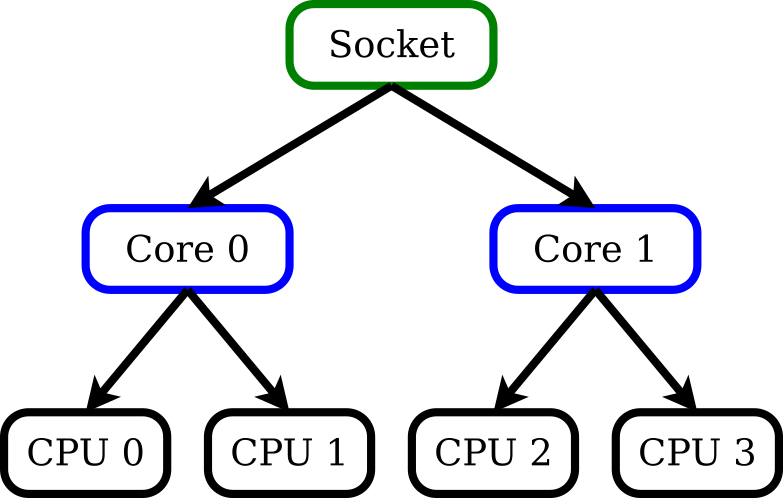
\includegraphics[width=4cm]{obrazky-figures/sched-domains}
  \caption{Hiearchy of scheduling domains}
  \label{fig:sched-dom}
\end{figure}

\section{Scheduling on SMP systems}
Symetric mutiprocessing (SMP) is an architecture of computer with multiple
physical processors, that have single shared memory, access to all IO devices
and run on the same instance of operating system. This allows the machine to
offer more processing power with a little overhead with memory sharing. Each
processor has still its own high speed cache, but with memory sharing there must
be maintained \emph{cache coherence} -- the uniformity of data shared between
processors in their caches.

For the main shared memory there are two ways of accesing it from multiple
processors: uniform (UMA) and non-uniform (NUMA) memory access.

\subsection{Uniform memory access}
In UMA architecture all processors share one memory controller they use to
access shared memory. Each processor has the same speed of memory access and
latency. They share one common access route to memory which brings more
simplicity at the cost of lower bandwidth and speed.

This architecture is easier for the scheduler to balance processes between
the physical processors. The time to access the shared memory is same on all of
the cores and there is no need to move the process memory to any other place for
faster access.

\subsection{Non-uniform memory access}
The problem with low bandwidth tries to solve the NUMA architecture.
It groups physical processors or group of cores with their own separate memory
and bus for faster access. This significantly improves overall memory throughput
of the system with correct utilization.

Nodes are also have to be connected to each other to access memory of other
nodes. That is achieved with interconnecting buses or even controllers. Each
manufacturer has its own technology implementing the interconnection
technologies: Intel uses Ultra Path Interconnect which replaced its QuickPath
Interconnect from older machines, AMD uses Infinity Fabric supersetting older
HyperTransport.

On bigger machines with larger amount of processors not every two processors are
connected, but access the data through a path of connected ones. This can be
seen on Figure \ref{fig:proliant} showing 8 NUMA node machine with advanced
structure of interconnect buses and controllers.

%Best Practices When Deploying Linux on DL980 4AA3-6556ENW.pdf
\begin{figure}
  \centering
  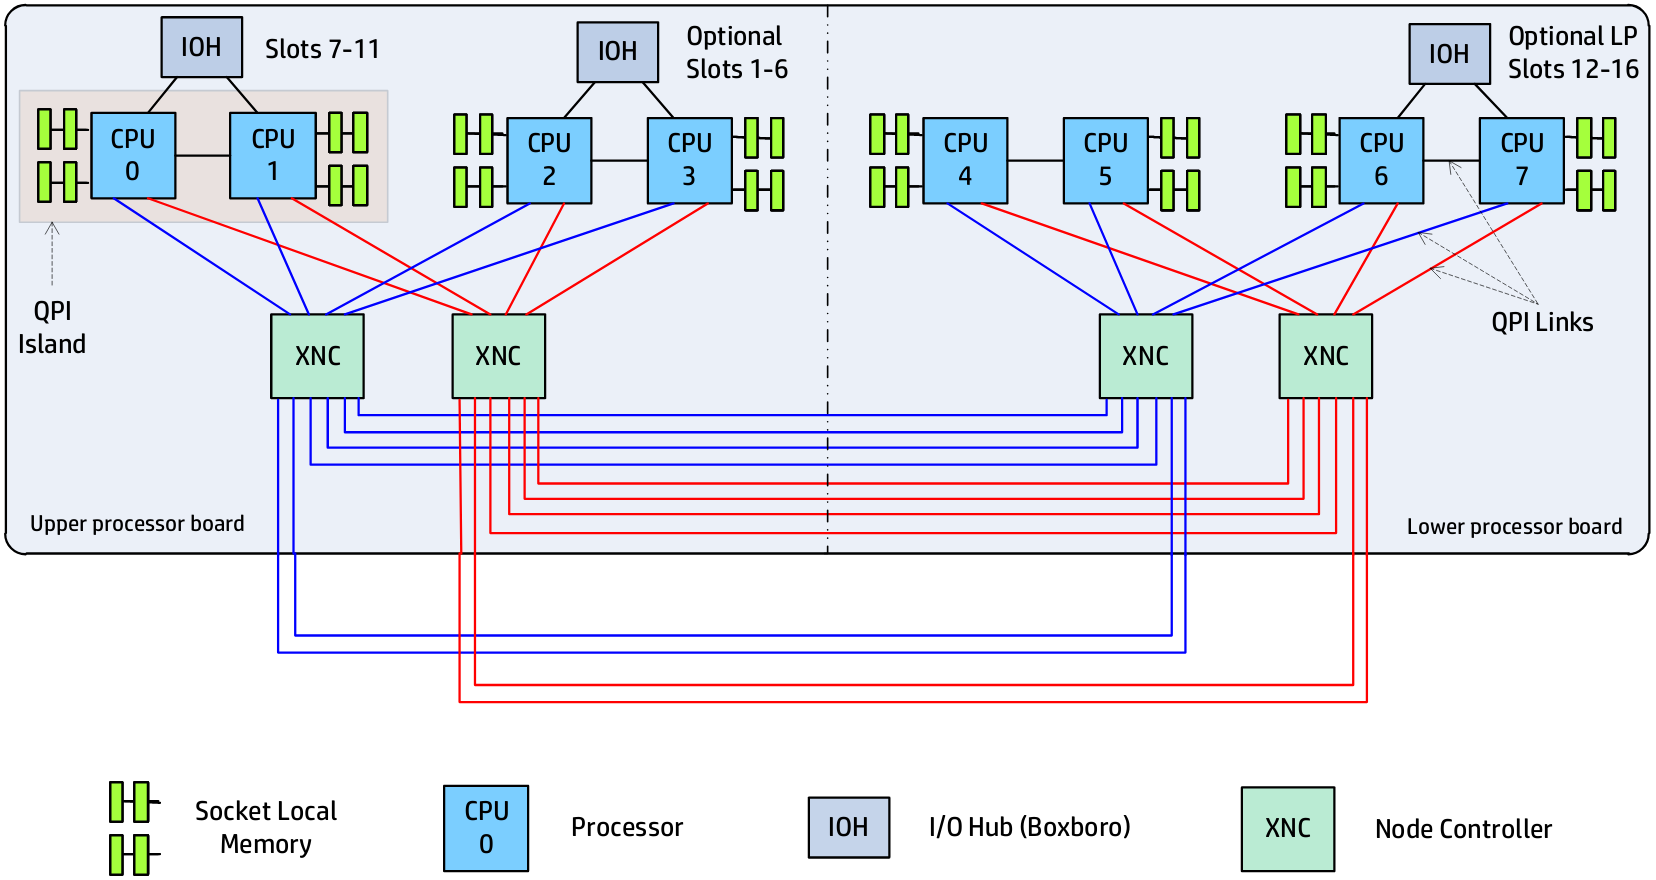
\includegraphics[width=14cm]{obrazky-figures/proliant}
  \caption{Architecture of NUMA communication on HP ProLiant DL980}
  \label{fig:proliant}
\end{figure}

Consequence of this is different latency between nodes which must be taken into
account when balancing tasks between nodes. Difference of access latency between
NUMA nodes for machine from Figure \ref{fig:proliant} shows part of output from
command \texttt{numactl --hardware}:

\begin{minipage}{\linewidth}
\begin{verbatim}
node distances:
node 0 1 2 3 4 5 6 7
0: 10 12 17 17 19 19 19 19
1: 12 10 17 17 19 19 19 19
2: 17 17 10 12 19 19 19 19
3: 17 17 12 10 19 19 19 19
4: 19 19 19 19 10 12 17 17
5: 19 19 19 19 12 10 17 17
6: 19 19 19 19 17 17 10 12
7: 19 19 19 19 17 17 12 10
\end{verbatim}
\end{minipage}\\

Balancing tasks between NUMA nodes is difficult for scheduler taking into
account expensive memory movement or access to different nodes. With wrong
approach the performance of NUMA system can even drop below the performance of
similar UMA system\footnote{http://highscalability.com/blog/2013/5/30/google-finds-numa-up-to-20-slower-for-gmail-and-websearch.html}.

Balancing processes between NUMA nodes is still in active development, which
brings many changes both to better or sometimes worse performance.


\chapter{Performance measurement}
Performance testing is examination of the system behavior under workload and its
effectivity of resource usage. Many systems depend on the time they are able to
respond and this property affects the usability of th system.

Compared to functional testing, performance testing does not produce exact true
or false result. It produces set of numerical values which must be compared to
pressumed values or values from other version to make a conclusion.

Next step is inspection of behavior of the system to understand the measured
values and determine the causes of the difference from the expected values.

For evaluation of system performance are usually used benchmarks.
Benchmarks generate artificial load imitating the load in real environment.
While stressing the system they also measure the performance. The benchmarks
typically return a value representing the performance of the system. The value
is usually in the form of the time that the task needed to finish or amount of
the operations that the system could perform per a unit of time.

Effectivity of task scheduling and of their migration between processors affects
the amount of the tasks that the system can handle and the time that a task
spends before finishing.

Although the benchmarks generate values that are suitable for comparison, they
do not provide any more detailed information about how the system achieved the
measured performance and where could be some possible bottlenecks.

To get a better insight into the behavior of the system, there are many tools to
collect information about the system behavior. Useful informations about the
scheduler include assignment of tasks to the processor cores, the time that the
tasks spent out of the CPU in queues, load of each processor core, and the
location of memory of the processes on NUMA systems.
% TODO cite http://www.brendangregg.com/activebenchmarking.html

\section{Performance metrics}
throughput

\section{Benchmarks}
In this chapter we will list the benchmarks that are currently used to evaluate
performance of latest kernel versions. The benchmarks are usually based on real
applications used both in scientific and business environments.

The benchmarks run in many threads or processes and feature communication
between the instances. With bad distribution of processes and threads by the
scheduler rises their time of waiting in the queue and the performance of the
system goes down. On NUMA systems performance depends moreover on placement of
data to the memory.

\subsection{NAS Parallel Benchmarks}
NAS Parallel Benchmarks is a set of benchmarks focused on performance of highly
parallel computations on supercomputers. In addition to floating point
computations, it targets communication and data movement among computation
nodes. The performed algorithms are based on large scale computational fluid
dynamics at the Numerical Aerodynamic Simulation (NAS) Program which is based at
NASA Ames Research Center.

Benchmarks are written in Fortran-90 or in C language, beacause these were the most
commonly used programming languages in scientific parallel computing community
at the time when the benchmarks were created. They can be compiled with different classes of
problem sizes to suit machines with different amount of memory and of computational
power.

Main output value of the benchmark is throughput measured in units called Mop/s
(millions of operations per second) representing amount of floating-point
operations per unit of time.

The benchmark also offers a few parameters that can passed to the benchmark
before the execution to tweak properties of behavior. One of them is a number of
computation threads, which in a lower amount slowers the run time, but allows to
measure behavior of the system without full usage. Figure \ref{fig:nas} shows
throughput with different number of threads on machine with 24 phisical cores
and Hyper-threading.

Downside of this benchmark is it can only run with fixed dataset, but not for a
fixed time period. This constraint makes the runtime of the benchmark with less threads longer

\begin{figure}
  \centering
  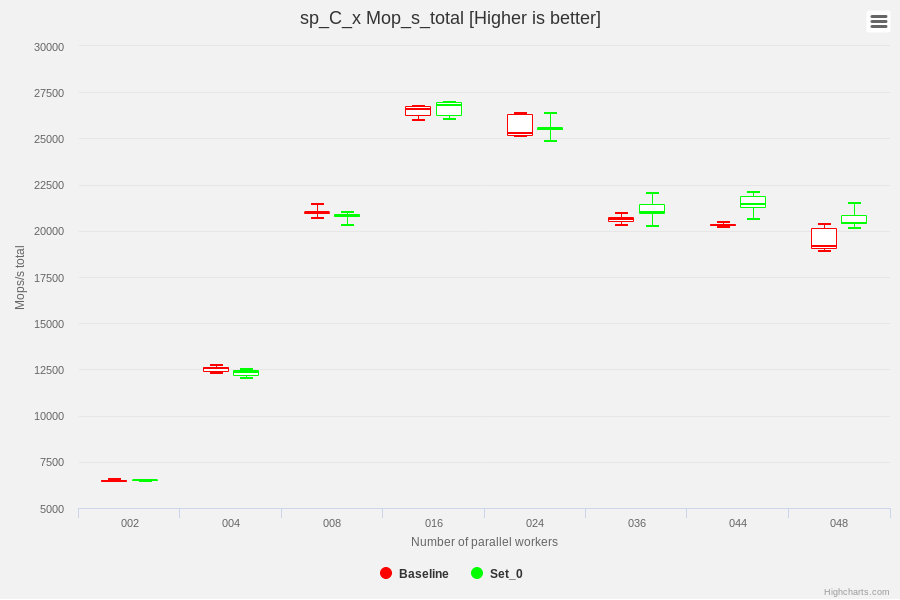
\includegraphics[width=12cm]{obrazky-figures/nas}
  \caption{Example of Scalar Penta-diagonal solver results from NAS Parallel with
    different number of computational threads.}
  \label{fig:nas}
\end{figure}

\subsection{SPECjbb2005}
Java Business Benchmark behaves as a server-side Java application. It is primarily focused on measuring performance of Java implementation, but also reflects performance of operating system and cpu itself.
It models system of wholesale company as a multitier application. The benchmark
itself creates the load, measures the throughput and also generates simple
report in HTML and raw text formats.

The main output value is \emph{throughput} in units called \emph{SPECjbb2005
  bops} \footnote{Business operations per second}.
In case of using more JVM instances, there is a second unit called SPECjbb2005
bops/JVM representing average throughput of single JVM\footnote{Java virtual machine} instance.
Another collected metric is memory comsumption, which isn't that useful in
scheduler performance monitoring.

\subsection{LINPACK benchmark}
LINPACK Benchmark comes from LINPACK package, wich was used to solve systems of linear equations in single or double precision.

\subsection{Stream benchmark}

\section{Performance analysis tools}

\subsection{time}
Time is a simple command for measuring the time that an application spent running. The
most common numbers it gives out are the total of real time that the application needed
to finish, the time that it spent in the user mode, and the time spent in the kernel mode.

Many benchmarks provide the execution time themselves which can make this
utility look useless. However the intersting information is the difference between
the userspace and the kernel time and the total execution time, which is time that
the application spent out of the CPU waiting in a queue.

It can be confused with bash builtin command \texttt{time}, which provides similar
information, but the real command can provide more verbose information with
a possibility of custom formating of output. It can be usually called from
\texttt{/usr/bin/time}.

\subsection{ps}
Ps is Linux command, which is used to display about active processes. Its name
stands for processes status. It can provide various information obtainable from
the virtual files in \texttt{/proc} directory. The most common information
include their PID, time spent on processor, state of the process, used memory,
associated terminal, the command that started the process and more.

Especially useful are optional columns \texttt{PSR} and \texttt{NUMA}. They
show the number of processor and the number of NUMA node where the process is
running. Continuous monitoring of those values can provide view on migration of
the process during its run time. 

Output of the command can be filtered in many ways. By default it shows only
processes from the current user and the current terminal, but it can list all
the processes on the system. The listing can be filtered using parameters by
most of the columns of information it provides. The listing can be limited for
instance by specific terminal, effective user, children of a specified process
or PID to single intended process.

\subsection{mpstat}

\subsection{turbostat}
This tool provides measuring of CPU usage and mainly its frequency.

\subsection{perf}


\chapter{Storing the results}
Benchmarks usually generate long human-readable output in text or even HTML
format. This is useful when analyzing single report. In the output are details
of the test run itself, simple resource usage or success of result validation.
However, the amount of result starts to rise with repeated runs, different
amount of instances and new versions kernels.

For the comparison of performance results, it is usually enough the number
representing throughput or time of each benchmark run. Those numbers can be
preprocessed from the benchmark output files to a format more suitable for quick
accesing required data.

\section{XML files}
XML is markup language, that can store heterogeneous data in tree structure.
However, the main feature of this format is human-readability. Even with the
inefficient storage of numerical data and repetition of tag and attribute names,
it allows user to quicky see the numbers without any processing of the data.

\section{Database}


\chapter{Displaying the results}
\section{Heat maps}
Heat maps are three dimensional graphs which are using color as the third
dimension for values. This allows to plot two dependencies of the values
compared to line graphs, which must use multiple lines to plot the same data.
Heatmapy škálují pro velké data. 
Data jsou kvantizovány do bucketů.

In the Figure \ref{fig:heatmap} is heat map showing utilization of all CPU cores over
time under workload. The data were collected by mpstat utility and processed to
show sum of user and kernel space utilization of each core. Plotting those data
using line graph with a line for every core would be confusing even for this
relatively small amount of CPUs.

\begin{figure}
  \centering
  \includegraphics[width=14cm]{obrazky-figures/heatmap}
  \caption{Example of heat map showing CPU utilization over time. The machine
    with 24 logical CPUs is under workload from NAS Parallel benchmark running
    in 16 threads.}
  \label{fig:heatmap}
\end{figure}

Another use of heat map is shown in Figure \ref{fig:numa_heatmap}. It does not
show utilization of threads, but their location on which NUMA node they are.
This heat map shows the migration of threads between NUMA nodes and the expected
result is not the highest value, but minimum of color changes in each line. The
shown data comes from NAS Parallel benchmark, which was run with 16 and 24
threads in 5 loops. The heat map shows better scheduler behavior on the 16
threads run than on the 24 threads run.

\begin{figure}
  \centering
  \includegraphics[width=14cm]{obrazky-figures/numa_heatmap}
  \caption{Example of heat map showing thread migration between NUMA nodes. The
    expected result is not the highest value, but minimum of color changes in
    each line. The shown result comes from machine with 24 logical CPUs running
    NAS Parallel benchmark on 16 and 24 threads in 5 loops.}
  \label{fig:numa_heatmap}
\end{figure}

\section{Boxplots}
Boxplot is method for displaying statistical properties of data groups. The
usually displayed values are minimum, 1\textsuperscript{st} quartile, median,
3\textsuperscript{rd} quartile and maximum.
This feature is useful to visualize accuaracy and reliability of measurement.
Then it's easier to distinguish performance regression from noise.

\begin{figure}
  \centering
  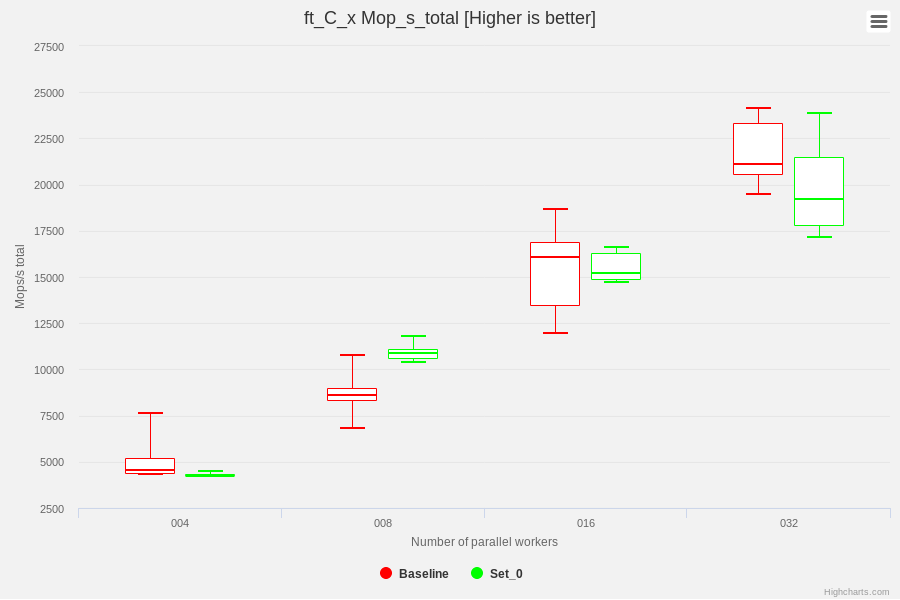
\includegraphics[width=12cm]{obrazky-figures/boxplot}
  \caption{Example of boxplot showing Mops of NAS benchmark with different
    number of threads}
\end{figure}


\chapter{Timelines}
An common way to get performance report is to compare two results. Usually, they
are called baseline and target results. The comparison of two results allows to
write many details about the measurement and changes between versions. Those
details usually contain clues to the cause of possible performance change.

However, sometimes is not enough to compare just two versions and larger amount
of results over longer period of time can bring a new perspective. There is much
more visible difference between the deviation from measurement error and the
performance change. It is also easier to find the versions, where a
performance degradation occured and where was fixed.

With larger amount of data, there can also emerge performance drops, which
appeared continuously over longer period of time and couldn't be spotted,
because they were in tolerance due to deviation.

\section{Result storage}
Benchmark results are stored on filesystem in directories. Each result consists
of two XML files with information and preprocessed main data from the test run,
more files with larger complementary data from analysis tools and compressed
original outputs from benchmark. First XML file contains metadata from the test
run including time, machine hostname, kernel and OS version, benchmark name,
configuration of environment, which could affect the result and few other data.
The second XML file contains the important preprocessed data itself.

The program has to go throgh all these results to choose the right ones for the
following creation of graphs.

\section{Comparison rules}
For automatic report generation are essential rules, which will specify results,
that can be used and in which role. I chose \emph{regular expressions} to match
properties of results. Regular expressions offer broad possibilities to describe
shape of kernel version or just value of any evironment configuration. To filter
all builds of kernel 4.18 works simple pattern \texttt{kernel-4.18\textbackslash
..*}.

To store the rules are stored in XML file with same node naming as in XML file
with result properties. The first level of XML document contains three nodes
representing purpose of rules.
\begin{itemize}
  \item \textbf{Baseline rules} specify the first result in plotted set. Acts as
    main result others are compared to.
  \item \textbf{Target rules} define the results to be plotted.
  \item \textbf{Starting rules} are for case, when base result is not from
    target set of results and specifying first target result with regex would be
    hard.
\end{itemize}
Each of theese nodes then contain in them nodes with the rules.


\chapter{Automatic evaluation}
With every expansion of regular kernel testing rises the amount of produced
results. With more machines with different configurations, benchmarks with
different focus or baselines from different supported versions, number of results
can rise with every new kernel version even by hundrets. This tends to automate
the repetitive classification of results between pass and fail to leave results
without significant change and focus on the ones with performance regressions.

\section{Marking of results}
To teach automatic classificator is essential large amount of data. To reduce
time spent on marking of the passed and failed results I created a form in
report to quicken this process.

On machine for storing results is running simple server application for
commiting requests from the form. The server is written in Python built on top
of Flask framework. On request it finds given result and modifies its file with
marking for learning.

\begin{figure}
  \centering
  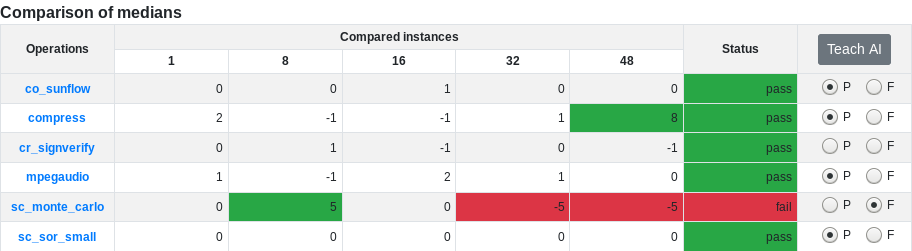
\includegraphics[width=12cm]{obrazky-figures/teaching_table}
  \caption{Form from HTML comparison report page to mark data for machine learning}
\end{figure}


%\chapter{Future work}


\chapter{Notes}
\begin{verbatim}
Linux scheduler
    CFS
    numa planning
        not easy for scheduler
        manual pinning option
            numactl
        group imbalance bug
    tune profiles
        focus on throughput or latency
Performance
    performance isn't simple pass/fail
    comparison of baseline and target kernel
    running just benchmark is waste of testing potential, it's good to collect more data
        http://www.brendangregg.com/activebenchmarking.html
    provisioning of machines with Beaker
    collecting system load data
        mpstat
            usage of every cpu
        numastat
        numatop
            usage of cpu and memory on each node
        ps
            psr and numa column
            cpu time
        time
            total, user and system time spent
        turbostat
        perf stat
        lstopo for hardware schema image
        free
    benchmarks
        specjbb2005
        specjvm2008
        nas parallel
        linpack benchmark
        stream (memory throughput)
        specjbb2015 - not stable
        hackbench - not tried yet
    scenarios
        variable number of benchmark instances
        with and without pinning processes to specific numa nodes
    result storing
        preprocessing to xml
        storing to database
        aggregating results
        computing statistical data
    plotting
        lstopo for plotting hardware topology
        bargraphs to show inaccuaracy
            operations per second (runtime of benchmark)
            time out of cpu
        detailed comparsion of two results
        timeline with many results over longer period of time
        heatmaps for core usage over time
            http://www.brendangregg.com/HeatMaps/utilization.html
        graph of process migration between numa nodes
Timelines
    analysis
    used technologies
    desing
    implementation
    output
Automatic regression detection
    motivation
    marking data
    preprocessing for classificator
    methods
        linear logistic regression
        decision trees
    evaluation
\end{verbatim}

\chapter{Specification}
\begin{enumerate}
\item Get acquainted with the existing methods for measuring performance of the Linux kernel scheduler and with means of storing of benchmarks results for further processing.
\item Study possible ways of processing these results with a focus on graphic interpretation and on methods for detection of performance degradation.
\item Design and implement a method for efficient graphic interpretation of long-term measurements.
\item Design and implement a method for automatic detection of performance regression.
\item Demonstrate the functionality of your implementation on at least two versions of the Linux kernel.
\item Evaluate the obtained results and discuss possibilities of further development of the project, especially of the automatic detection of performance regression.
\end{enumerate}

Literature:
\begin{itemize}
\item Lozi, Jean-Pierre, et al. "The Linux scheduler: a decade of wasted cores." Proceedings of the Eleventh European Conference on Computer Systems. ACM, 2016.
\item Daniel, P., and Cesati Marco. "Understanding the Linux kernel." (2007).
\item Bailey, David H., et al. "The NAS parallel benchmarks." The International Journal of Supercomputing Applications 5.3 (1991): 63-73.
\end{itemize}
